In this section, we learn about functions.  Mathcad has a large library of built-in functions (logarithms, trigonometric functions, statistical functions, etc), but we can create new functions as well.  

\section{Mathcad: Built-in Functions}\label{sec:Mathcad_functions}

\index{Mathcad!Function Listing}
To access the complete list of built-in functions in Mathcad, use the menu with Insert $>$ Function or type Ctrl + e.

\begin{center}
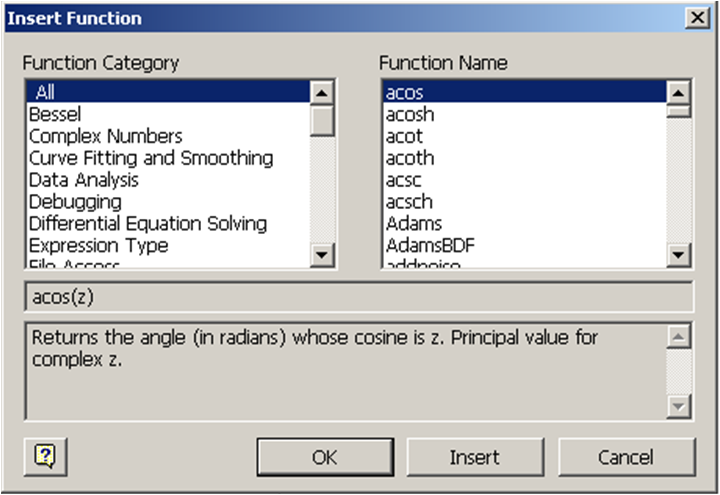
\includegraphics{figures/mathcad_function_dialog_box.png}
\end{center}

Selecting a ``Function Category'' (left side of the dialog box) will restrict the list under ``Function Name'' (right side of the dialog box) for easier searching.  A description of the highlighted function's output will appear in the lower part of the dialog box.

A few special functions that one might use often:\\

\index{Mathcad Functions!square root}
$\bullet$ \textbf{Square root}\\

The square root function can be created either using the Calculator toolbar or by simply typing $\backslash$.  To create an $n$th root, also in the Calculator toolbar, the shortcut key is Ctrl + $\backslash$.\\

\index{Mathcad Functions!absolute value}
$\bullet$ \textbf{Absolute value}\\

Both bars in the total absolute value symbol are created at the same time when selected from the Calculator toolbar (the $|\textrm{x}|$ button), or by typing the vertical bar $|$ (located on your keyboard above the Enter key - it looks like two stacked bars, but will create one solid vertical bar).\\


\keyidea{idea:absvalVSdet}{\textbf{Absolute Value versus Matrix Determinant}\\
If you already know about determinant of matrices:\\ 
The determinant and the absolute value look exactly the same on the page (both are $|\textrm{x}|$) and both are created using the same keyboard shortcut key (the vertical bar~$|$~)! \\ 
If you have an error using the vertical bars, it could be that you are either trying to take the absolute value of a matrix (not allowed), or the determinant of a number (not allowed either). You have to be very careful as to the context of your problem in using these two functions!}

\section{Mathcad: User-Defined Functions}\label{sec:Mathcad_functions2}

\index{Mathcad!User-defined Functions}
\noindent \large \textsf{\textbf{User-Defined Functions}} \normalsize\\

Sometimes you will need to create your own function in Mathcad, perhaps for repeated use throughout a worksheet.  The syntax looks very similar to the way a function might appear in a math textbook.  The function name is followed immediately by the input variables (in parentheses and separated by commas), a definition equals sign (colon), and then the expression in terms of the input variables.  When the function is executed, the input variables are replaced with constants, including units as desired, and followed by the evaluation equals sign. Consider the following example.\\

\example{ex_userfunction1}{{\bf Create a function for the volume of a cylinder}\\
\\
The function, called \textbf{Volume}, is defined in terms of the variables \textbf{radius} and \textbf{height} (don't forget to use the assignment equals, created with a colon :).\\
\\
\tnr{Volume(radius,height):=$\pi$ radius$^2$ height}\\
\\  
The symbol for $\pi$ can be created on the Greek toolbar, or with the keyboard shortcut Ctrl + Shift + p.  Now, when we want to compute with the function, we substitute values for radius and height (including any unit) into the function\\
\\
\tnr{Volume(2ft,3ft):= $1.068 \times 10^3$} \tnr{L}\\
\\
or\\
\\
\tnr{Volume(500cm,2000cm):= $1.571 \times 10^6$} \tnr{L}\\
\\
Note that Mathcad converts to the metric unit L (liters) as default.
}

\newpage
\printexercises{exercises/13_exercises}